\chapter{SENSOR MEASUREMENTS}\label{cha:measurements}
In this chapter the methods used for testing the mobile devices for different characteristics is described in~\chapterref{cha:character}.Three different test where performed to get sensor data to analyze for bias and characteristics. \\
\\
Overview of the tests performed:
\begin{itemize}
  \item[] \textbf{Motion sensor measurement I:} Aimed to collect the data via a web-page since JavaScript can access \textit{gyroscope} and \textit{accelerometer}.
  \item[] \textbf{Motion sensor measurement II:} Second test was implemented as an Android application to also measure sensor readings from \textit{gyroscope} and \textit{accelerometer} with the addition of the \textit{magnetometer} together with some adjustments in the approach of the measurements.
  \item[] \textbf{Motion sensor measurement III:}

  \item \textbf{Camera measurement I:} Collect one video from each device and extract pictures frames from the video. Calculate and compare the PRNU of the extracted pictures.
  \item \textbf{Camera measurement II:} Collected photographs instead of video from the device to get more sensor information. 
\end{itemize}

\section{Motion sensor measurement I: Web-page ``Gyrotion''}\label{sec:measurement:gyrotion}
Developed a web-page to collect the accelerometer and gyroscope data that JavaScript provide (~\sectionref{subsec:accJS}).  The web-page is called ``Gyrotion'' due to it measures gyro and motion.
This only require that the measured device has Internet connection and a browser installed, no additional installations and completely cross-platform.\\
\\
The measurements required that the device where still on a flat surface, then started by pressed a button. It gathered 1000 samples of accelerometer and gyroscope data that then where saved as a CSV for further analyzing. The screen-shots below shows the web-page while measuring and the right one when finished and ready to send. 
\begin{figure}[H]
  \hspace{-2cm}
  \centering
  \begin{minipage}[c]{.23\textwidth}
    \centering
    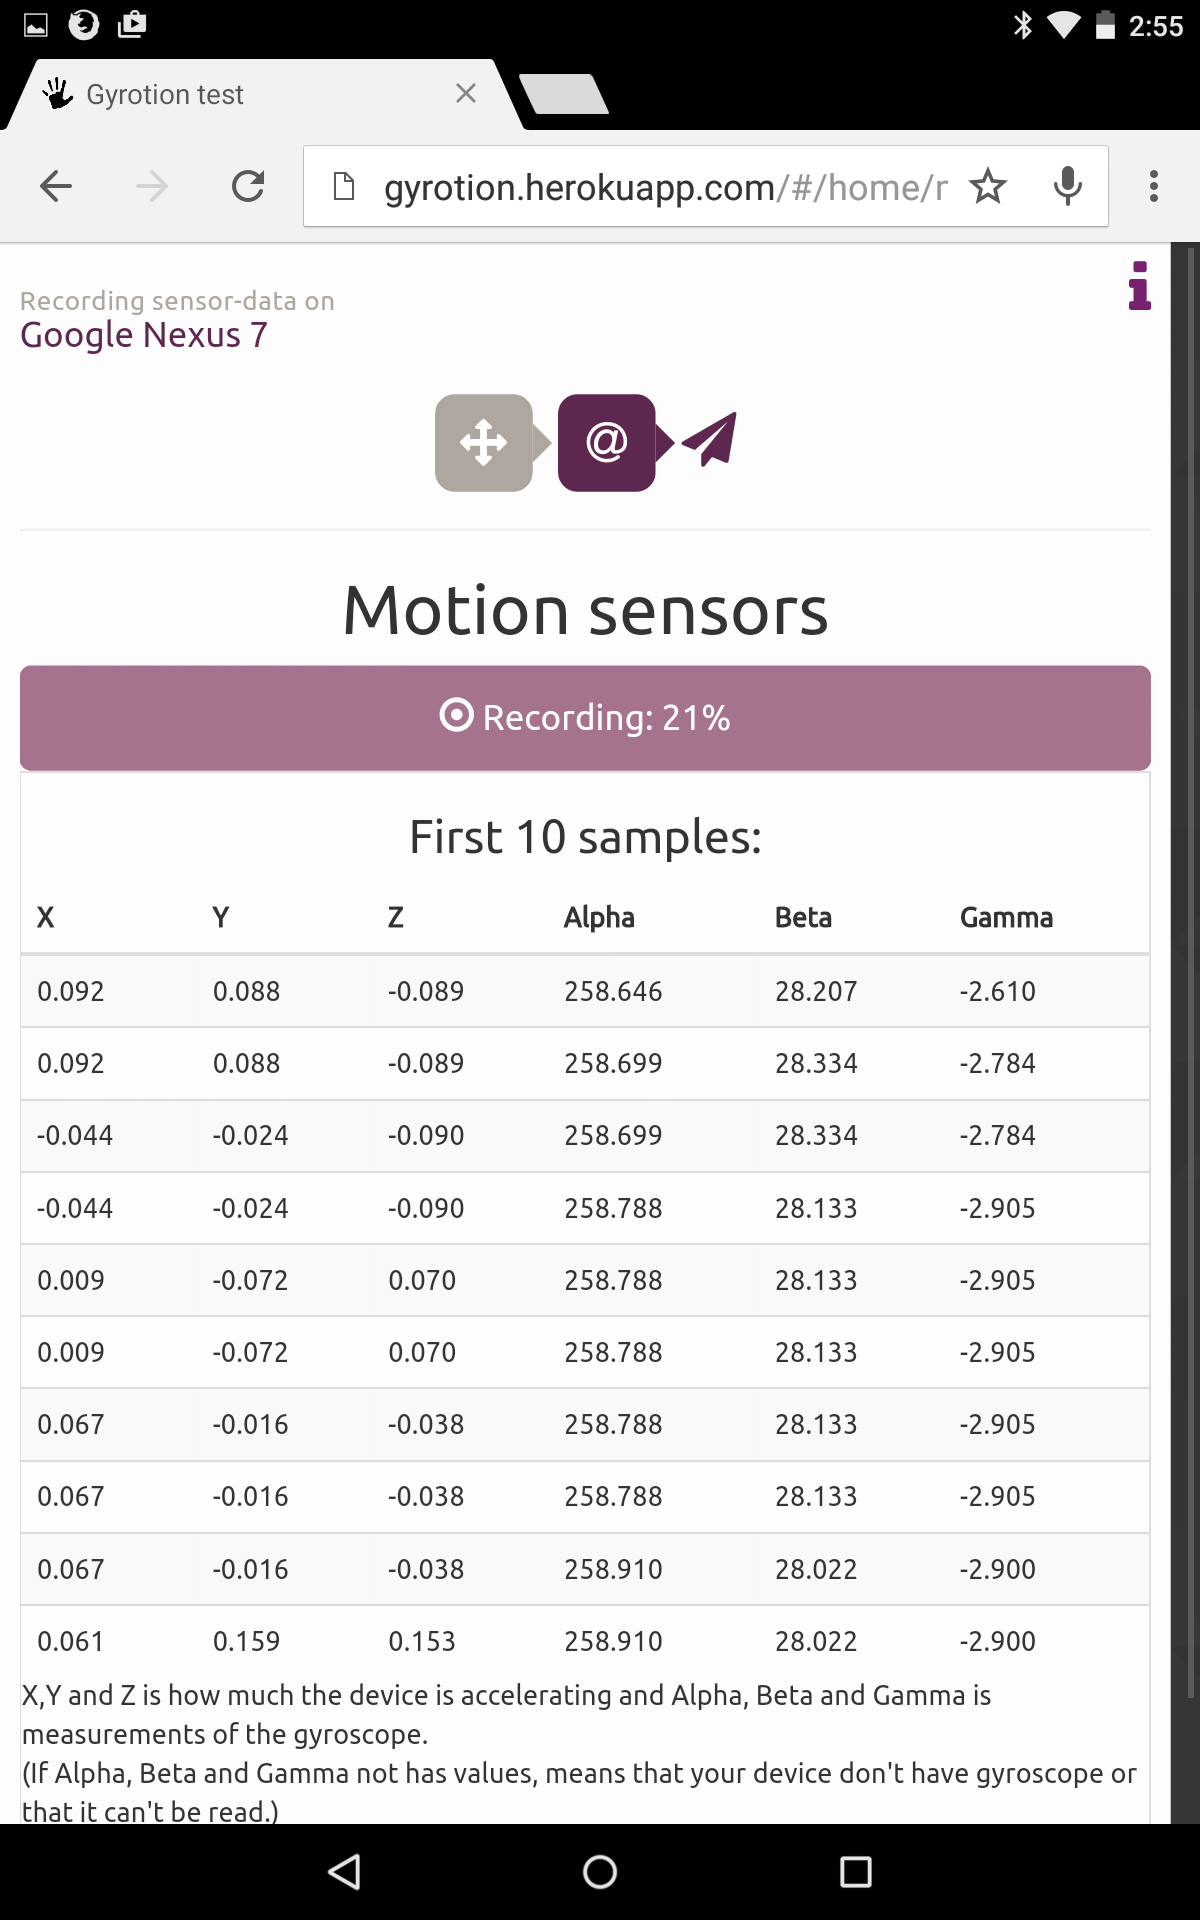
\includegraphics[scale=0.1]{img/Nexus-rec}
  \end{minipage}
  \hspace{2cm}
  \begin{minipage}[c]{.23\textwidth}
    \centering
    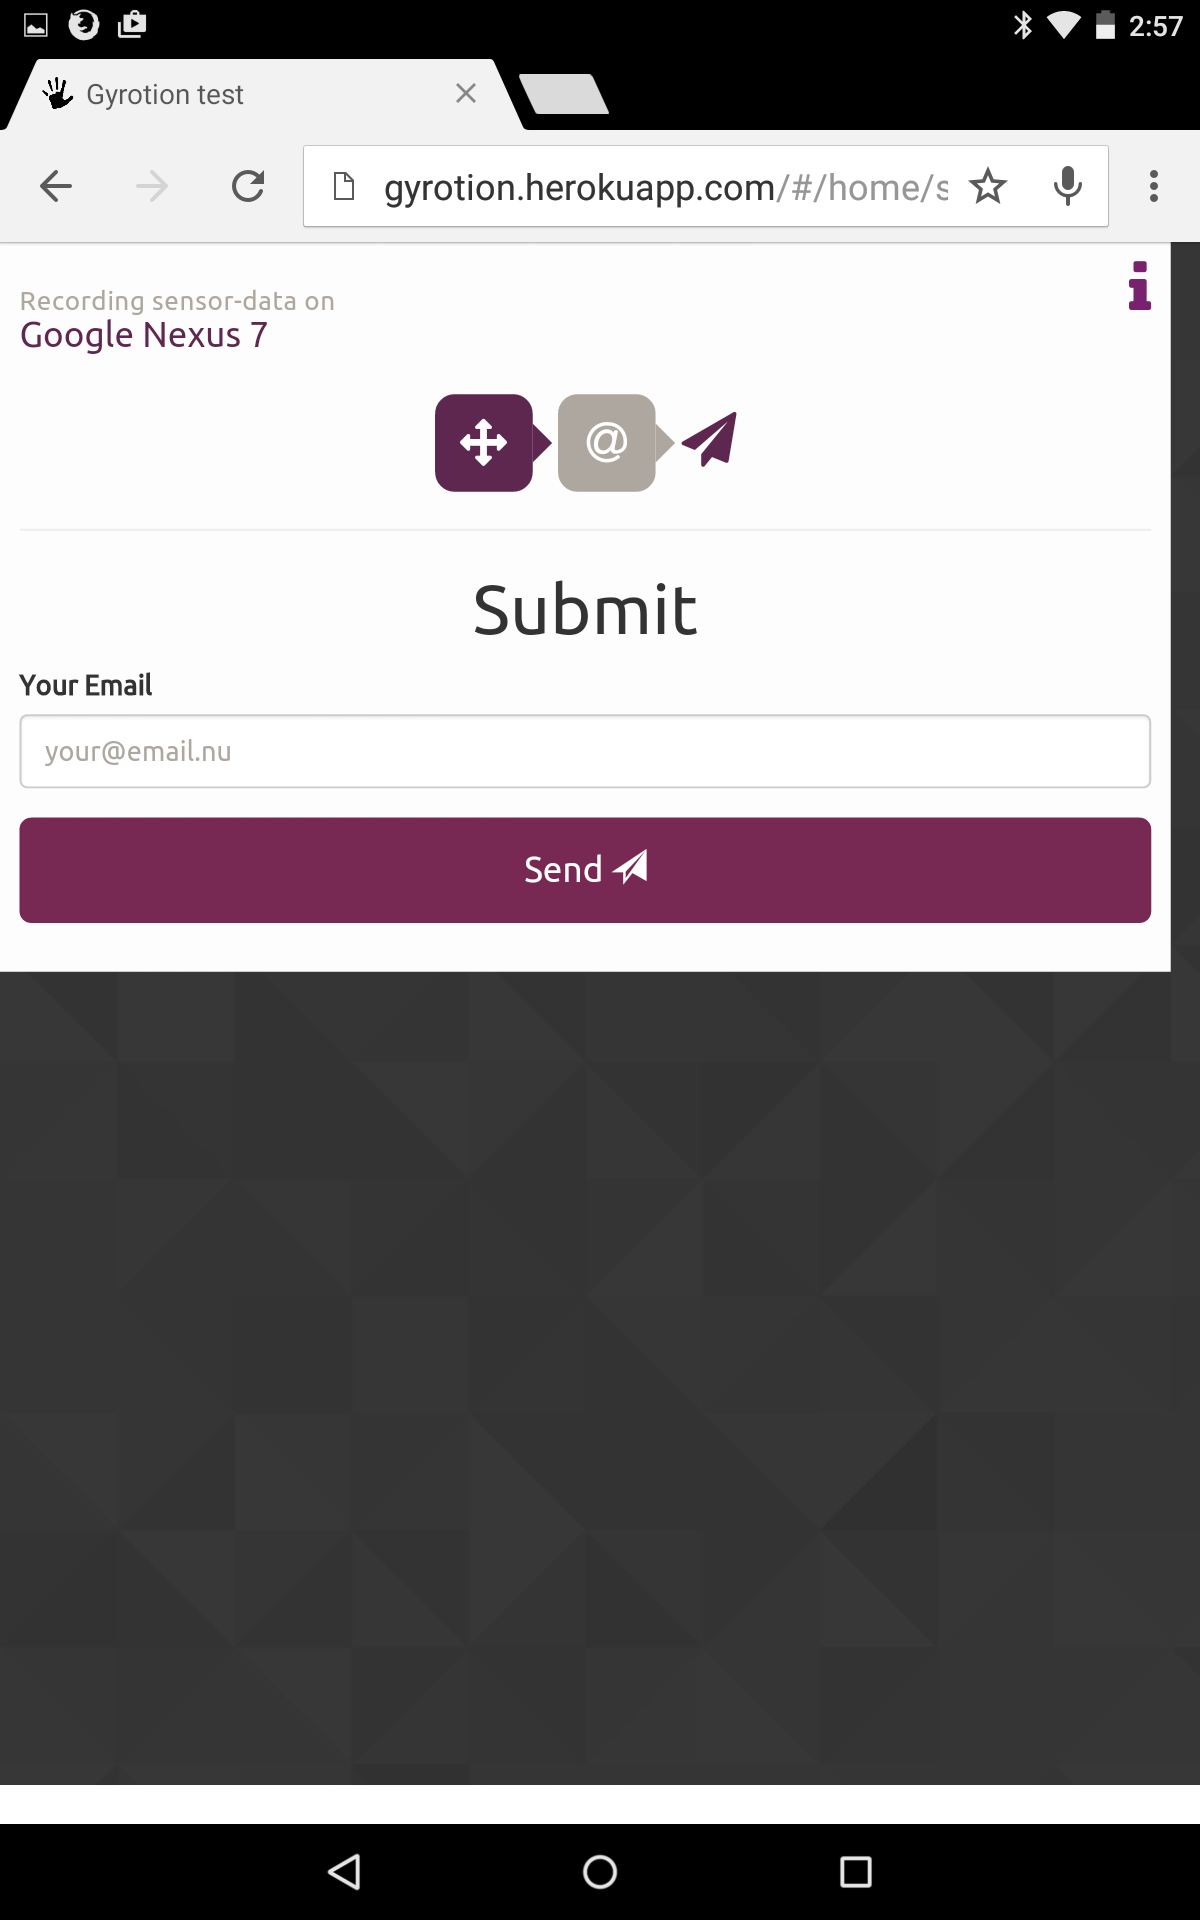
\includegraphics[scale=0.1]{img/Nexus-submit}
  \end{minipage}
  \caption{Screen-shots of motion sensor measurements on web-page ``Gyrotion''}
  \label{fig:gyrotion}
\end{figure}

\section{Motion sensor measurement II: Web-page ``SensorRec''}\label{sec:measurement:sensorrec}
Since added camera to the test the name ``Gyrotion'' no longer where applicable it became ``SensorRec'' (short for sensor recordings)
From the last test some changes were made to improve the test result:
\begin{enumerate}
  \item Adding time-stamp to every recording sample to know exactly recording frequency to enable further analyzing.
  \item Time based recording on 30 seconds instead of taking 1000 samples as in the first test (~\sectionref{sec:measurement:gyrotion}).
  \item It's also sampling at a lower rate of at least 10 ms instead of as fast as it could before to reduce the effect of other processes that may are in use on the device.
  \item Also switch the accelerometer listener from \texttt{acceleration} to \texttt{accelerationIncludingGravity}, since I suspect that that will give more raw accelerometer data, thus less bias removal by Android and JavaScript. 
  \item Added a step for video recording, more about that in~\sectionref{sec:measurement:camera}.
\end{enumerate}
\begin{figure}[H]
  \hspace{-2cm}
  \centering
  \begin{minipage}[c]{.23\textwidth}
    \centering
    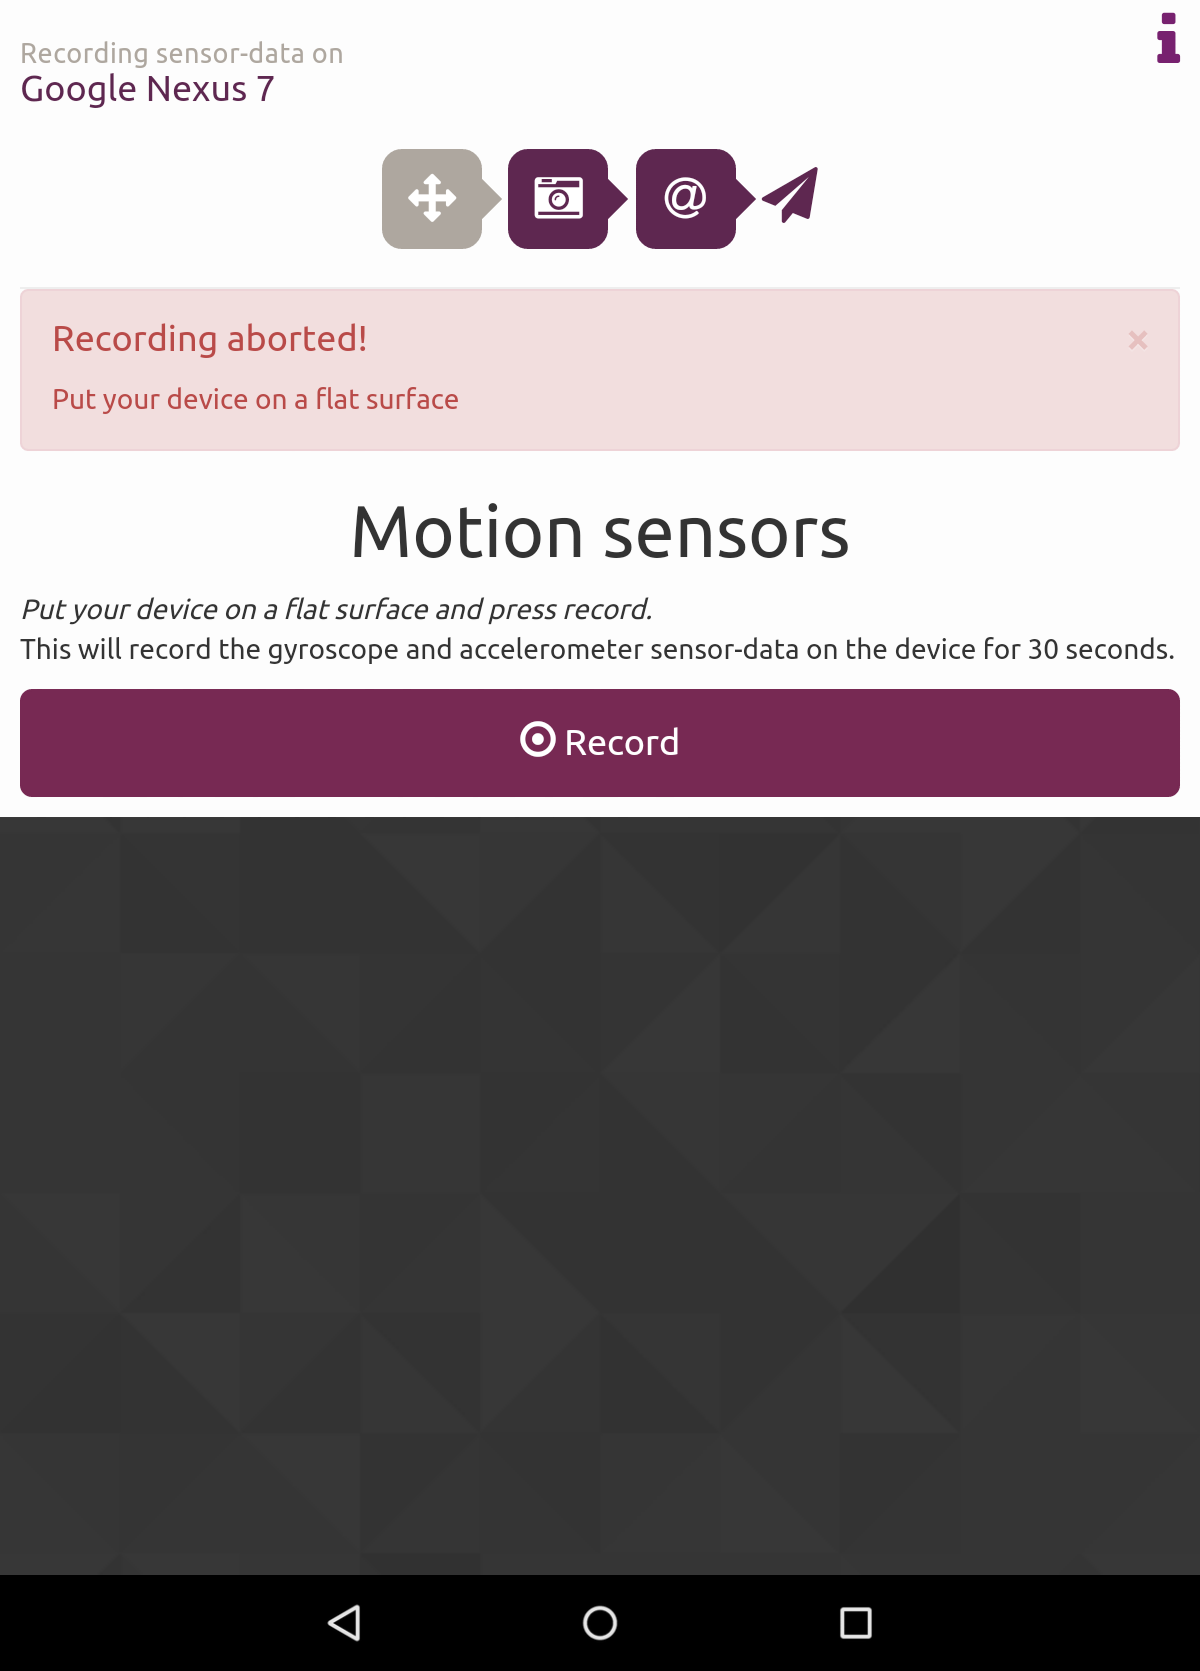
\includegraphics[scale=0.15]{img/sensorrec-nexus-2-notRec}
  \end{minipage}
  \hspace{2cm}
  \begin{minipage}[c]{.23\textwidth}
    \centering
    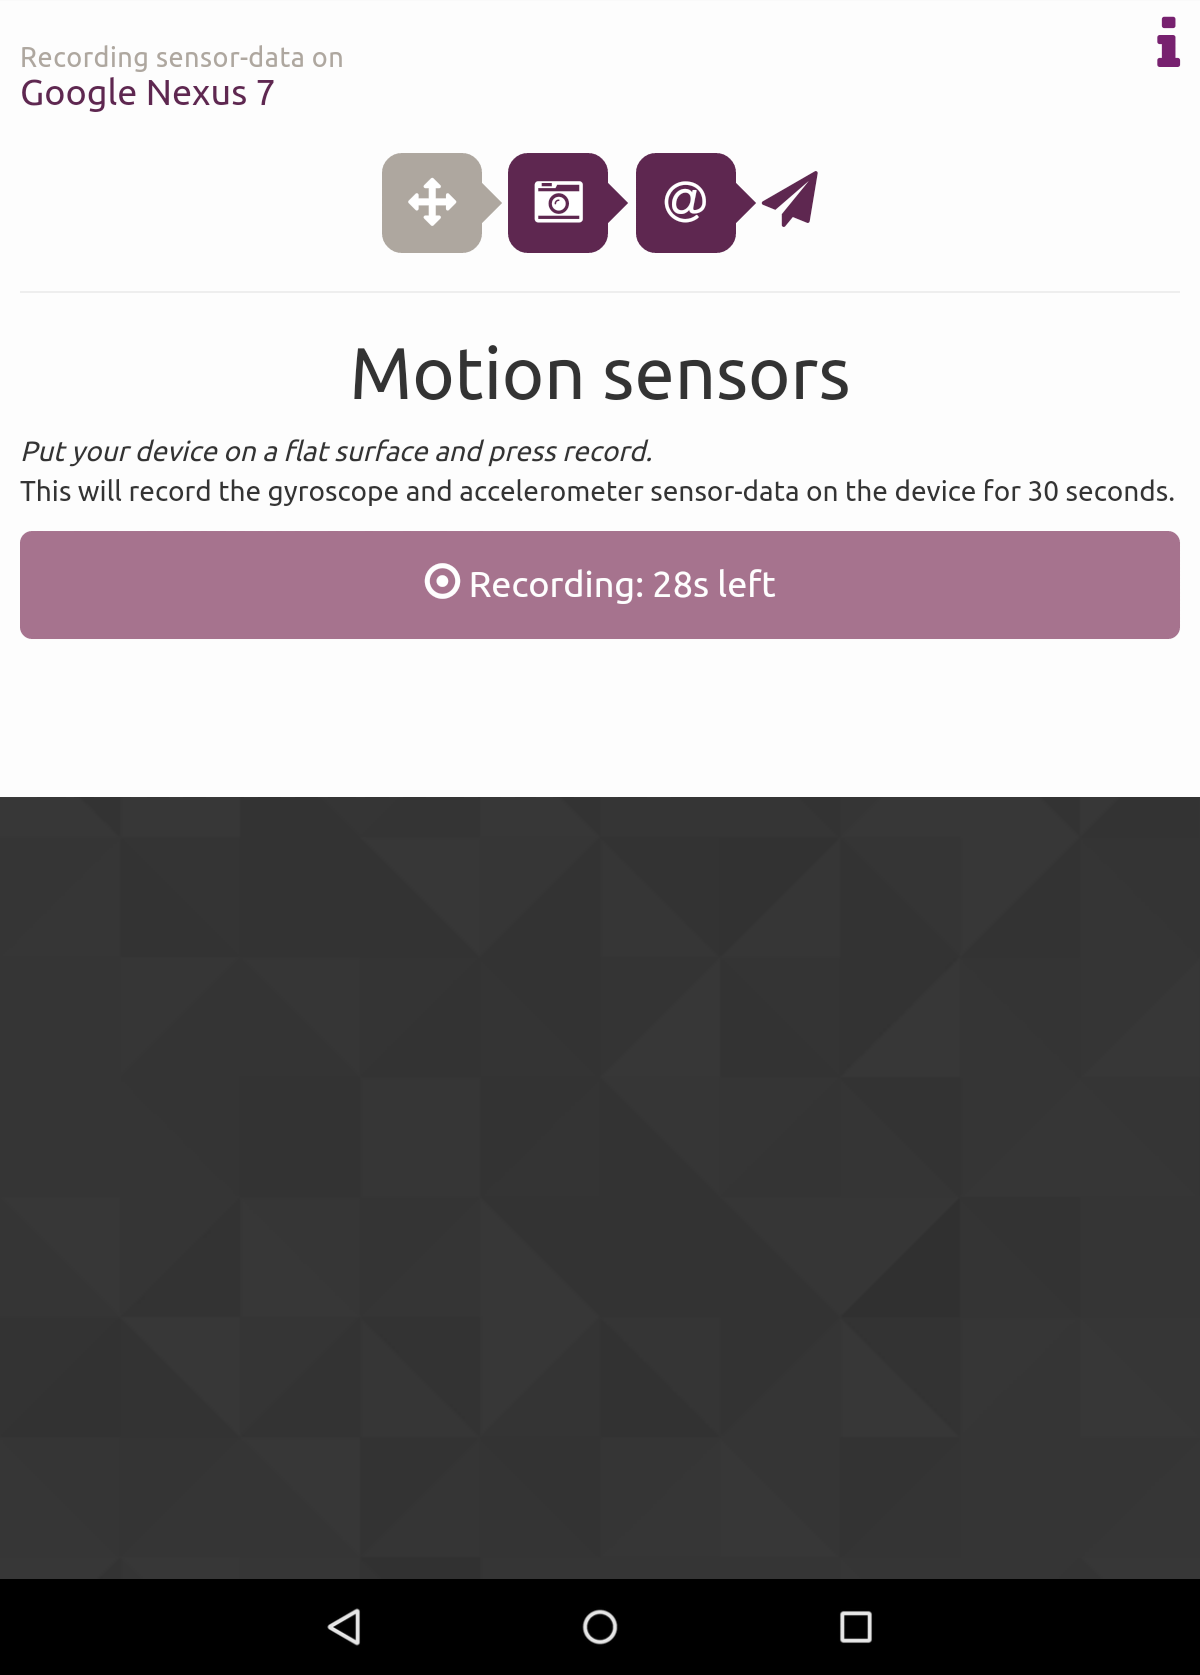
\includegraphics[scale=0.15]{img/sensorrec-nexus-1-rec}
  \end{minipage}
  \caption{Motion sensor measurements II on a Google Nexus 7}
  \label{fig:sensorrec}
\end{figure}
The link for this page where spread and XXX measurements where made. The page is online on address: \url{http://sensorrec.herokuapp.com}

\section{Motion sensor measurements III: Android application}
\textbf{ ==== OBS!! ====}\\
Kanske flyttar denna till demo-delen beroende på hur det går... och då får jag inte gömma att flytta Android o JavaScript från kap3 till ``rätt ställen'' \\
\begin{enumerate}
  \item An additional recording with the device placed in hand to make the measurements more diverse bias estimation. 
  \item Make 2 recordings with the difference of a 180 degree rotation alpha wise (see \figureref{fig:device-axes}) for better bias estimation \cite{acc:kionixerr}. REMOVE?
  \item Added ``Morse''-vibration in the recording to remove environmental bias which is one of the largest sources of bias ~\cite[p.8]{acc:kionixerr}. The ``Morse''-vibration is a test pattern of Morse that the device vibrated like during the measurements. The reason for this is to have data for the demonstration (REF TILL IMPLEMENTATION!!) of challenge response-authentication made by the device.
\end{enumerate}
\textbf{ ==== OBS!! ====}\\
Lägga till lite scceenshots o kod o grejer...

\section{Camera measurements}\label{sec:measurement:camera}
As most of the camera fingerprinting articles (REFERENSER!!) the aim has mostly been forensic and not focusing on the measurability or integrity of the pictures. That is why some limitations has been made in these measurements, e.g. black-motive (integrity) and not as large amount of picture required (measurability). \\
To measure the camera two measurements where gathered in both cases where the device on a flat surface which makes the camera result black. Both of this measurements is analyzed by the PRNU-method used by~\cite{sensor:camera:DCIdent} described in~\sectionref{sec:ResCam}.
\begin{enumerate}
  \item \textbf{Black video:} The recommended number of pictures for camera fingerprinting is 50 ~\cite[]{sensor:camera:DCIdent}. But that is not a convenient gathering purposes, thus to ask someone to take 50 black photos and send will not make many answers. Thats why the first test asked for recording a 5 seconds video-recording with the camera towards a flat surface. This video is then shuttered into picture frames, 5 seconds generate 100-200 pictures depending on the recording rate of fps (frames per second).
  \item \textbf{10 black photos:} Simple as taking 10 photos, also with the camera pointing down on a flat surface. Since ~\cite{sensor:camera:DCIdent} where using pictures of diverse motive this aims to investigate if there may be enough with 10 pictures when the motive is the same.
\end{enumerate}

Screen-shots from the camera-page of ``SensorRec'':
\begin{figure}[H]
  \hspace{-2cm}
  \centering
  \begin{minipage}[c]{.23\textwidth}
    \centering
    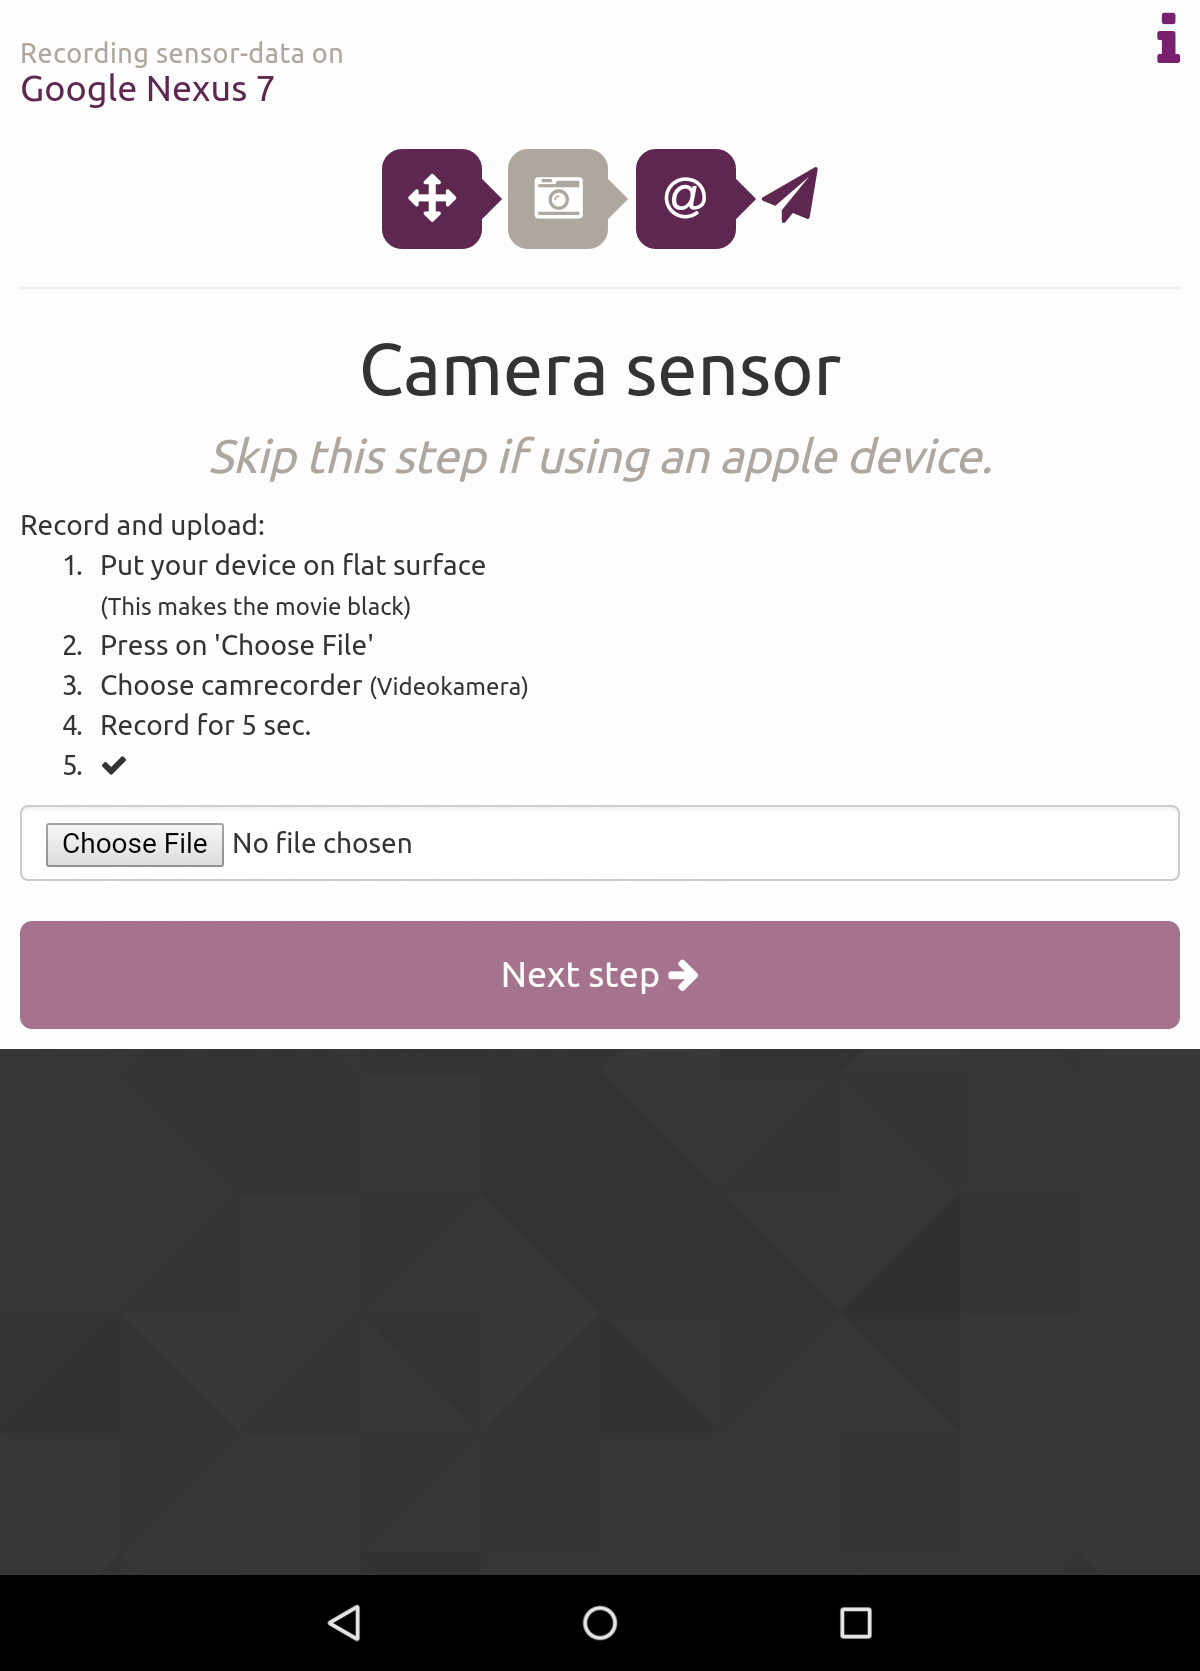
\includegraphics[scale=0.15]{img/sensorrec-nexus-3-cam}
  \end{minipage}
  \hspace{2cm}
  \begin{minipage}[c]{.23\textwidth}
    \centering
    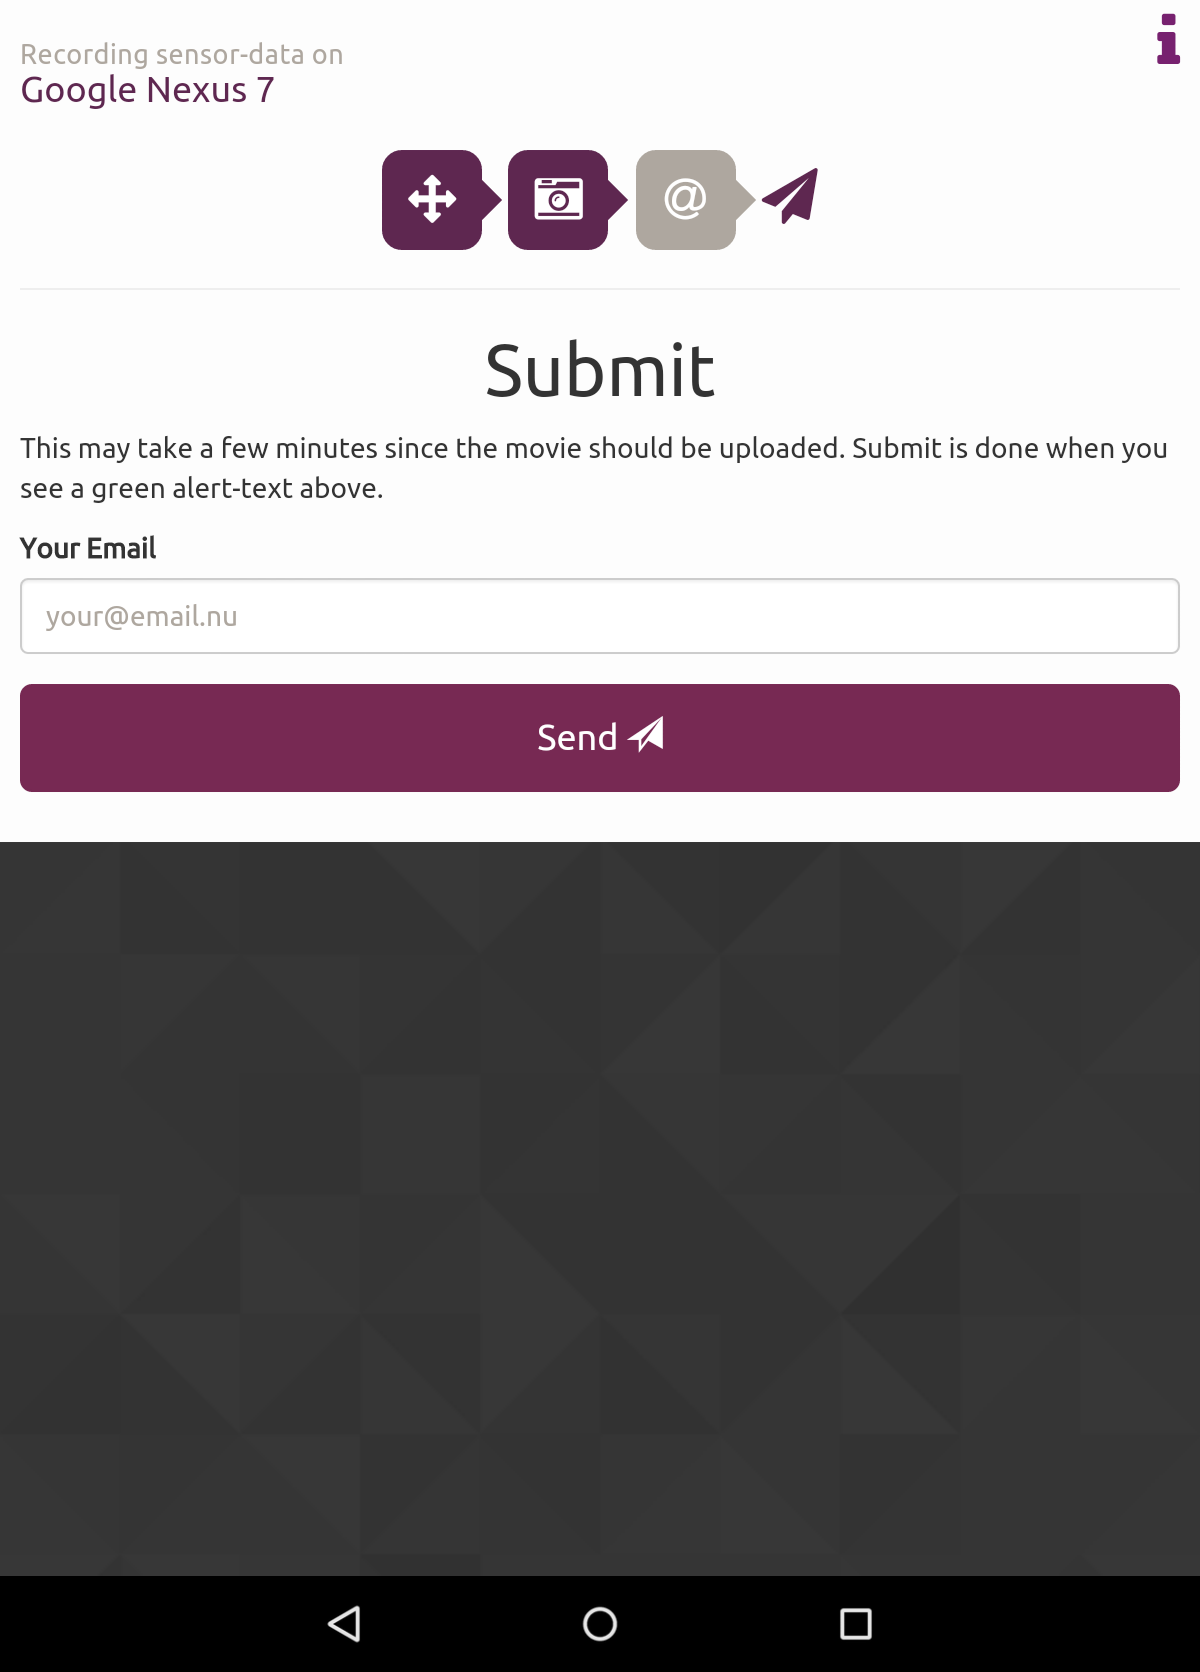
\includegraphics[scale=0.15]{img/sensorrec-nexus-4-send}
  \end{minipage}
  \caption{Sensor measurements on a Google Nexus 7}\label{fig:sensorrecCamera}
\end{figure}